% Created 2025-03-11 Tue 15:00
% Intended LaTeX compiler: lualatex
\documentclass[bigger]{beamer}
\usepackage{amsmath}
\usepackage{fontspec}
\usepackage{graphicx}
\usepackage{longtable}
\usepackage{wrapfig}
\usepackage{rotating}
\usepackage[normalem]{ulem}
\usepackage{capt-of}
\usepackage{hyperref}
\usetheme[progressbar=foot, sectionpage=none, numbering=fraction]{metropolis}
\usepackage{tikz}
\usepackage{booktabs}
\usepackage{adjustbox}
\usepackage{diagbox}
\usepackage{latexcolors}
\usetikzlibrary{automata, positioning, arrows, arrows.meta}
\usepackage{diagbox}
\usepackage{dsfont}
\usepackage{amsmath}
\usepackage{fontawesome}
\usepackage{pgfgantt}
\usepackage[ruled]{algorithm2e}
\usepackage[absolute, overlay]{textpos}
\usepackage{xcolor}
\definecolor{UmlBlue}{HTML}{0067b1} \setbeamercolor{progress bar}{fg=UmlBlue} \setbeamercolor{title separator}{fg=UmlBlue}
\setbeamercolor{progress bar in head/foot}{fg=UmlBlue} \setbeamercolor{progress bar in section page}{fg=UmlBlue} \setbeamercolor{alerted text}{fg=UmlBlue}
\pretocmd{\tableofcontents}{\thispagestyle{empty}}{}{}
\usepackage{multimedia}
\usetheme{default}
\author{Andrea Pierré}
\date{March 11, 2025}
\title{Lab meeting}
\subtitle{\emph{Robust representations for olfactory-spatial association learning}}
\setbeamercovered{transparent=10}
\setbeamertemplate{section in toc}[sections numbered]
\AtBeginSection[]{\begin{frame}[plain, noframenumbering]{Outline}    \setbeamertemplate{section in toc}[sections numbered]\setbeamertemplate{subsection in toc}[subsections numbered]\tableofcontents[currentsection, currentsubsection]\end{frame}}
\AtBeginSubsection[]{\begin{frame}[plain, noframenumbering]{Outline}\setbeamertemplate{section in toc}[sections numbered]\setbeamertemplate{subsection in toc}[subsections numbered]\tableofcontents[currentsection,currentsubsection]\end{frame}}
\definecolor{headercolor}{HTML}{232323}
\setbeamercolor{normal text}{%
% bg=,
fg=headercolor
}
\hypersetup{
 pdfauthor={Andrea Pierré},
 pdftitle={Lab meeting},
 pdfkeywords={},
 pdfsubject={},
 pdfcreator={Emacs 29.4 (Org mode 9.7.19)}, 
 pdflang={English}}
\begin{document}

\maketitle
\begin{frame}[plain]{Outline}
\tableofcontents
\end{frame}

\section{Project recap}
\label{sec:org905dd1d}
\begin{frame}[label={sec:orgfc7c6df}]{The LEC is key to sensory associations and spatial memory}
\begin{columns}
\begin{column}{0.45\columnwidth}
\footnotesize
\begin{itemize}
\item \alert{Piriform Cortex} encodes olfactory information
\item \alert{Hippocampus} encodes spatial information
\item \alert{Lateral Entorhinal Cortex (LEC)} encodes both olfactory \& spatial information
\end{itemize}
\end{column}
\begin{column}{0.55\columnwidth}
\begin{center}
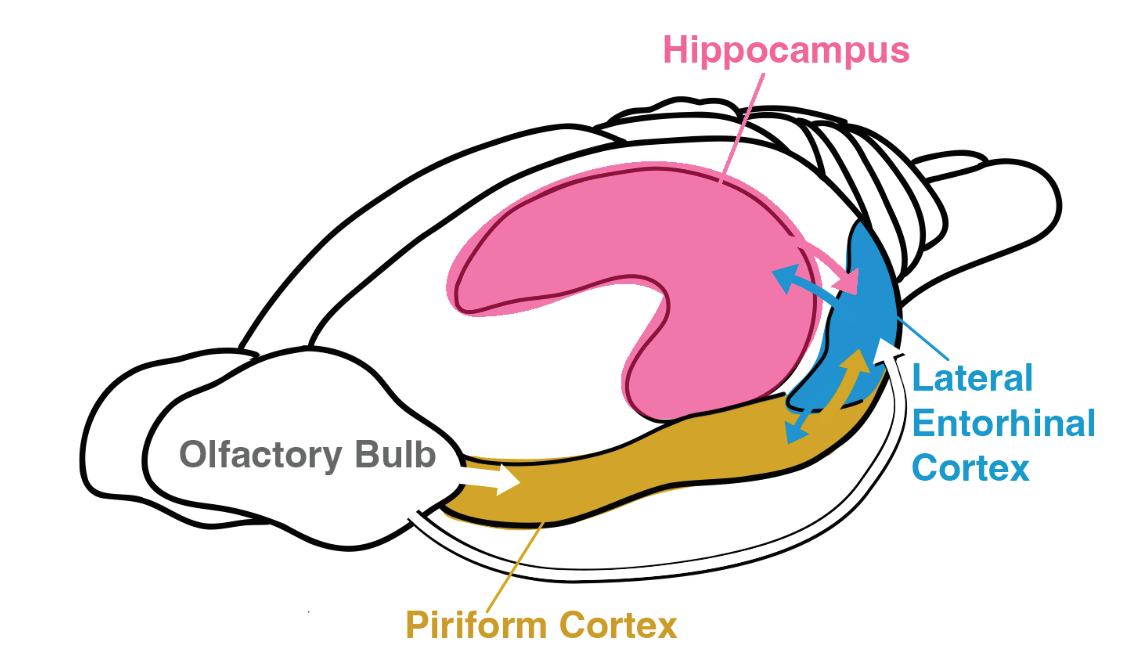
\includegraphics[width=\textwidth]{medias/brain.png}
\end{center}

\begin{textblock}{5}(0.5,14.5)%
\tiny
Poo et al., 2022\\
Bitzenhofer et al., 2022\\
Lee et al., 2021
\end{textblock}
\end{column}
\end{columns}
\end{frame}
\begin{frame}[label={sec:org1c1d836}]{Half triangle task for olfactory-spatial association learning}
\begin{columns}
\begin{column}[c]{0.33\columnwidth}
\begin{center}
\movie{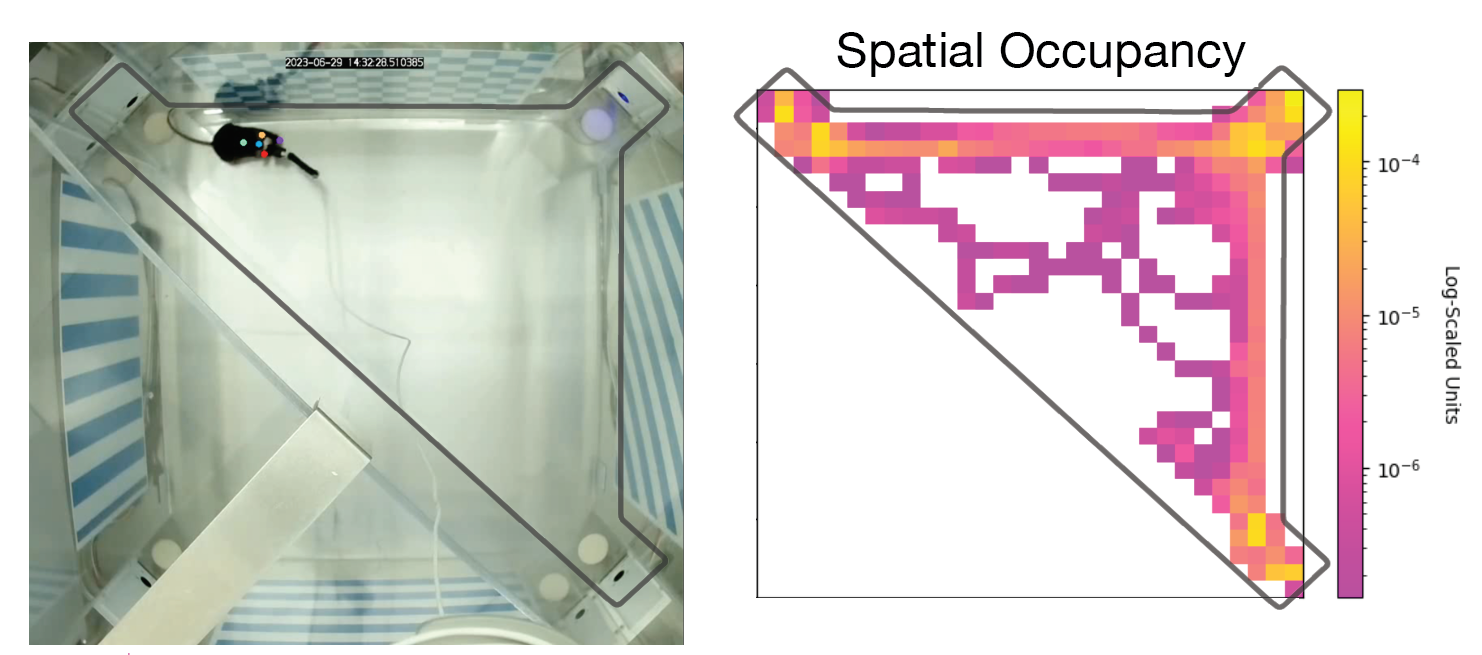
\includegraphics[width=\linewidth, keepaspectratio, trim={0cm 0cm 28cm 0cm}, clip]{medias/video-picture.png}}{medias/annotatedF03_d35_2022-11-15_15.41.mp4}
\end{center}
\end{column}
\begin{column}[c]{0.33\columnwidth}
\begin{center}
East/West task
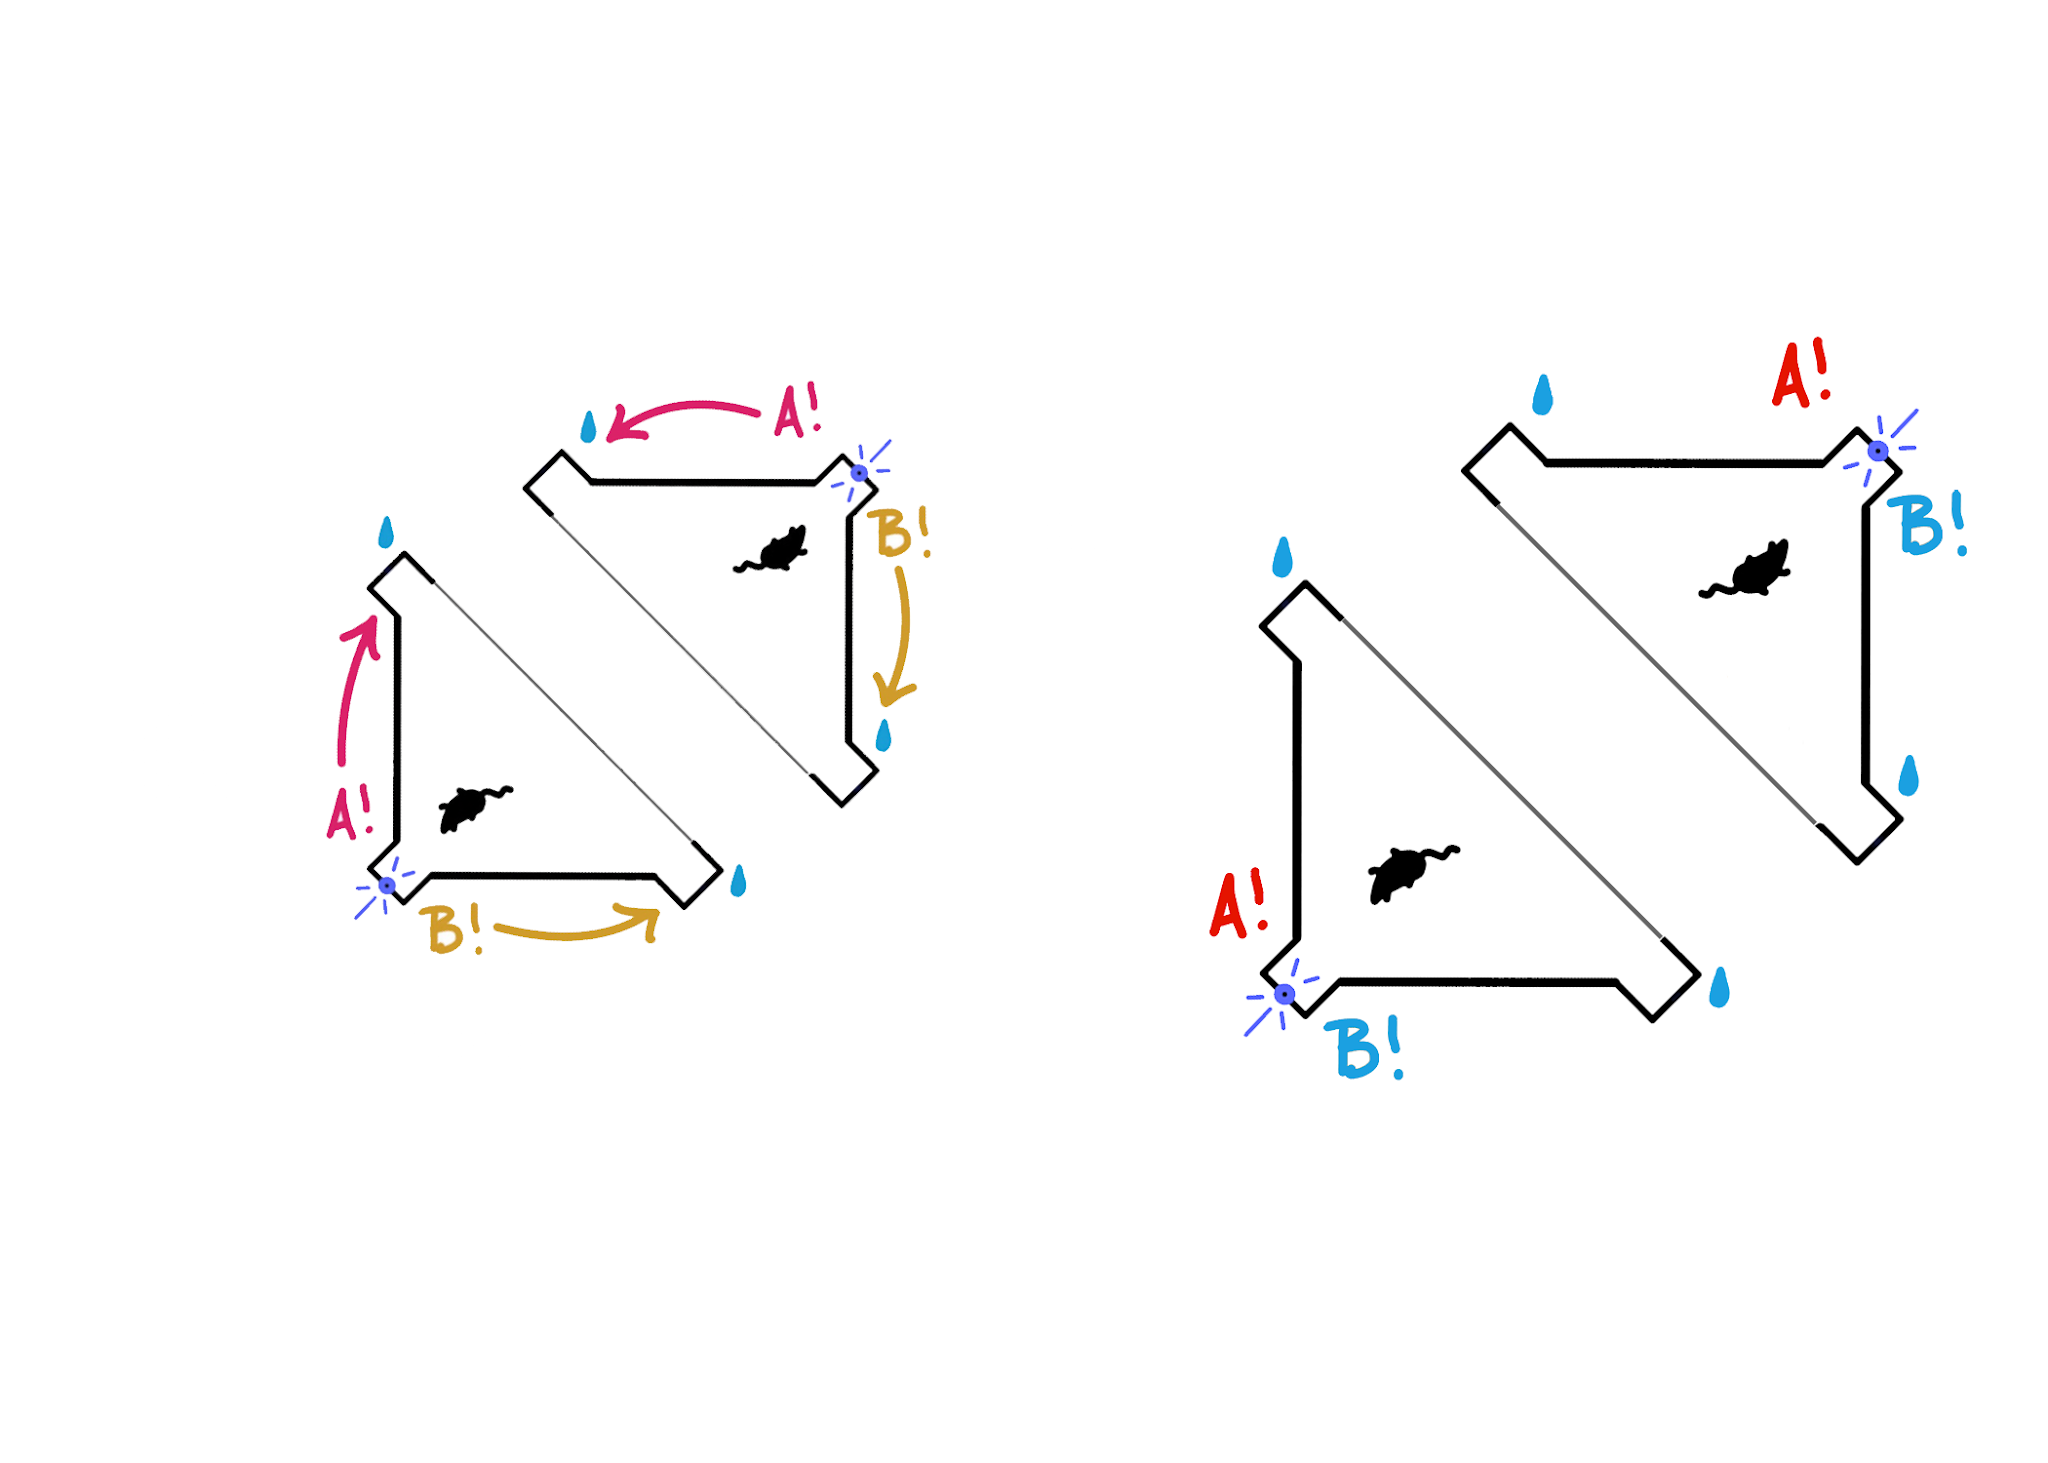
\includegraphics[width=0.9\linewidth, keepaspectratio, trim={11cm 18cm 40cm 13cm}, clip]{medias/task-east-west.png}
\end{center}
\end{column}
\begin{column}[c]{0.33\columnwidth}
\begin{center}
Left/Right task
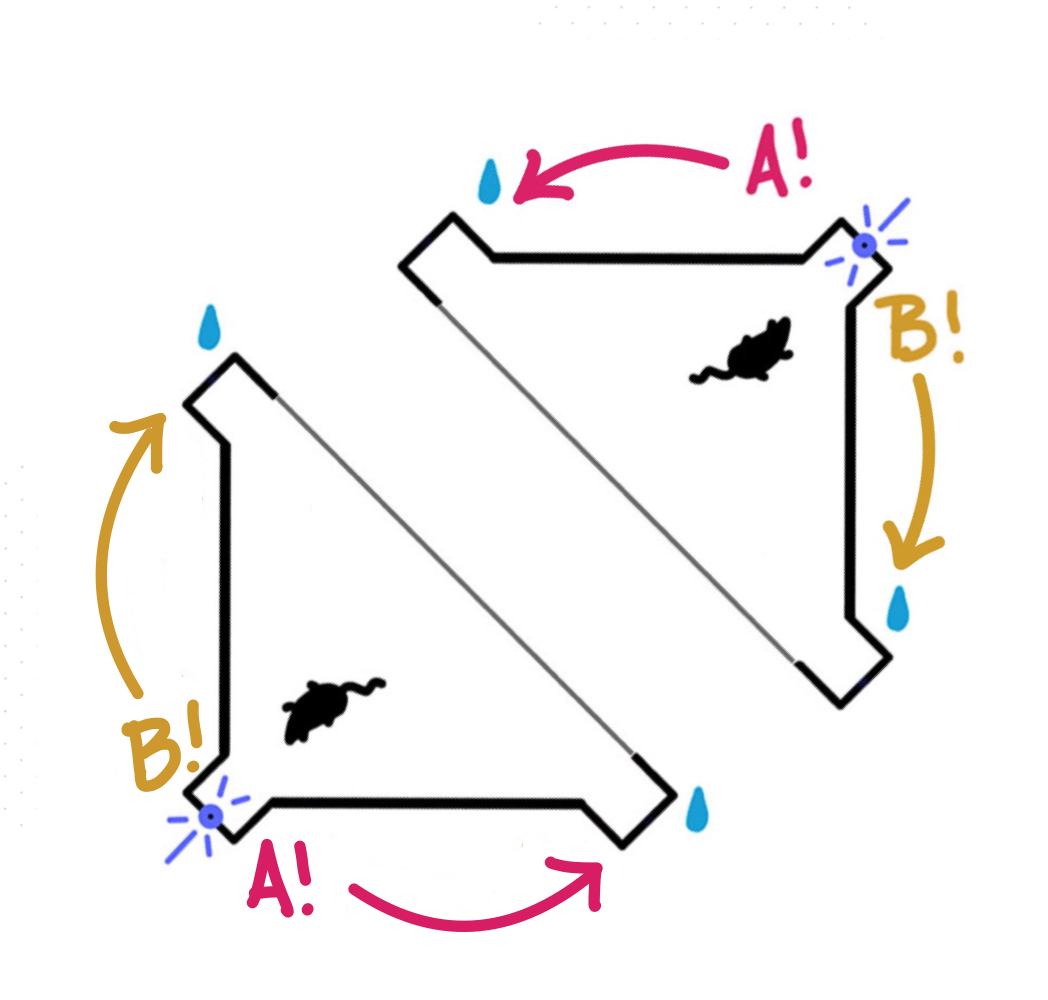
\includegraphics[width=0.9\linewidth, keepaspectratio, trim={3cm 2cm 4cm 4cm}, clip]{medias/task-left-right.jpeg}
\end{center}
\end{column}
\end{columns}
\end{frame}
\begin{frame}[label={sec:orgb774cac}]{Deep Reinforcement Learning model}
\begin{center}
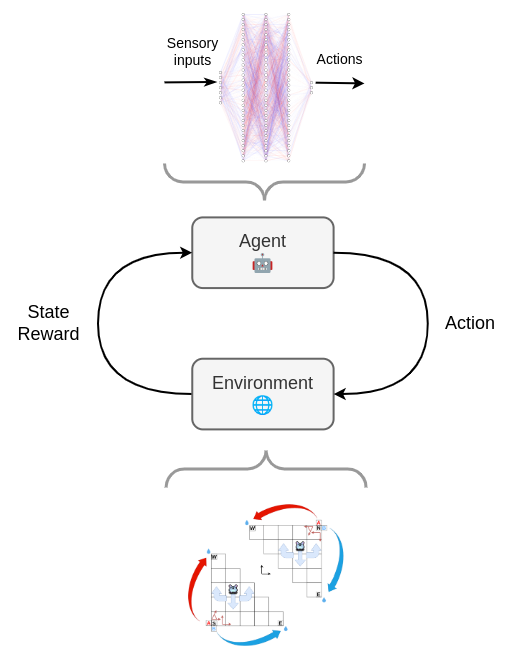
\includegraphics[height=0.95\textheight]{medias/nn.drawio.png}
\end{center}
\end{frame}
\begin{frame}[label={sec:org731b50e}]{The environment}
\begin{center}
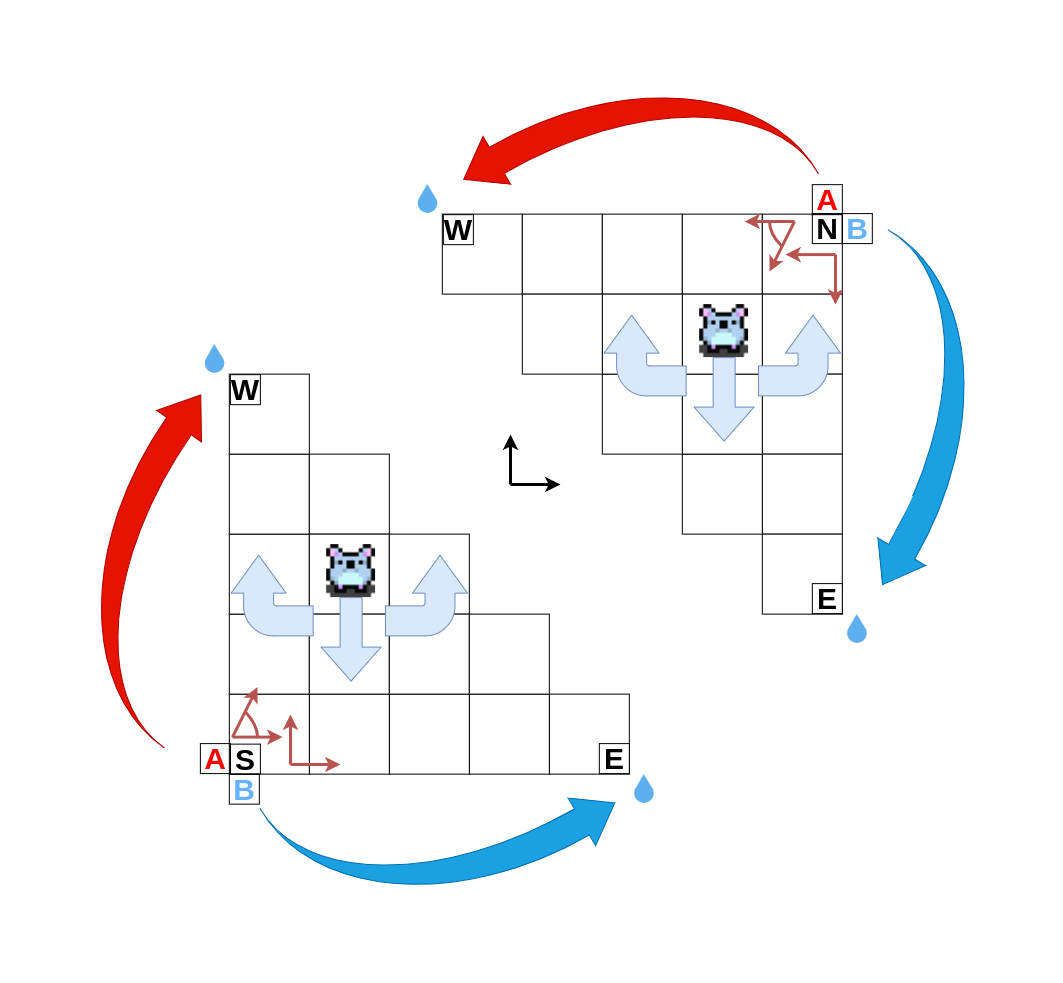
\includegraphics[height=0.6\textheight]{medias/RL_env-cartesian-polar.drawio.png}
\end{center}
\footnotesize
\vspace{-1em}
\begin{itemize}
\item 3 actions: \(\Leftarrow \quad \Uparrow \quad \Rightarrow\)
\item Duplicated coordinates inputs:
\begin{itemize}
\item Cartesian coordinates from north \& south port
\item Polar coordinates from north \& south port
\end{itemize}
\end{itemize}
\end{frame}
\begin{frame}[label={sec:orgc99888e}]{Questions \& Hypothesis}
\metroset{block=fill}
\begin{exampleblock}{Questions}
\begin{itemize}
\item What \alert{function} does the network learn?
\item How the constrains of the task affect learning \& the representations learned?
%\item How this task structure might employ different representations of the action space?
\item How do the representations learned compare between the \emph{in vivo} and the \emph{in silico} neurons?
\end{itemize}
\end{exampleblock}
\pause
\begin{exampleblock}{Hypothesis}
\begin{itemize}
\item The network will use the most efficient coordinate information based on the task
\item The structure of the network's weights will reflect this prioritization of information
\end{itemize}
\end{exampleblock}
\end{frame}
\begin{frame}[<+->][label={sec:orgab139ce}]{Looking back\(\dots\)}
\footnotesize
\begin{center}
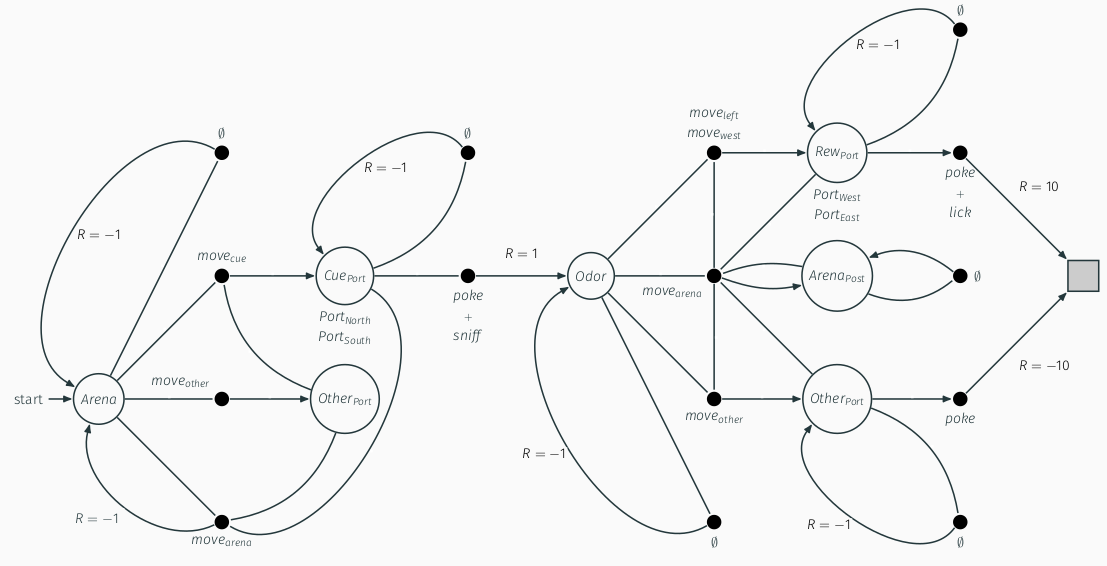
\includegraphics[height=0.45\textheight]{medias/mdp.png}
\end{center}
\begin{enumerate}
\item First step trying to define Olivia's experiment as a Markov Decision Process (MDP) in Julia
\item 2D tiles with tabular RL \& function approximation in Python/NumPy
\item 2D coordinate system in Python/PyTorch
\item Duplicated coordinates experiment in Python/PyTorch
\end{enumerate}
\end{frame}
\section{Modeling \& Simulation}
\label{sec:org281e3c6}
\begin{frame}[label={sec:orgf9594af}]{State space \& network architecture}
\begin{center}
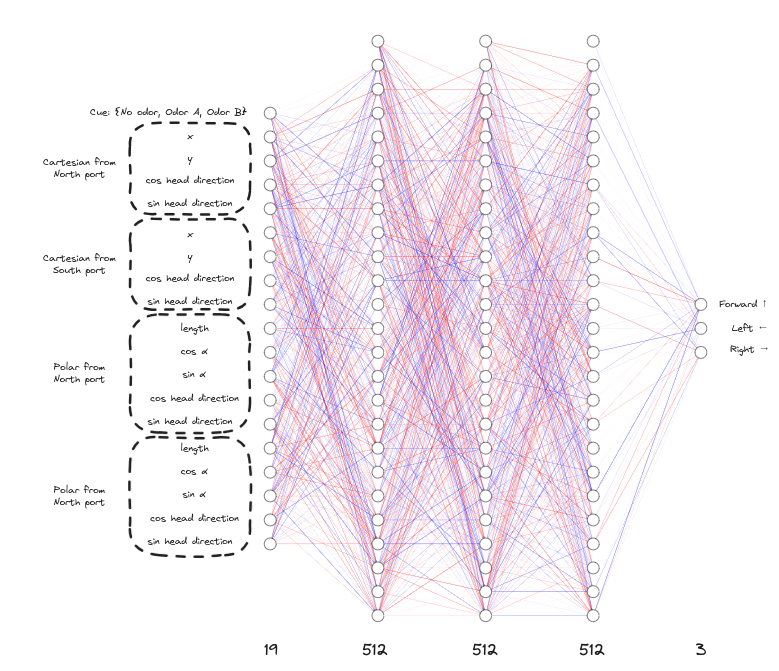
\includegraphics[height=0.97\textheight]{medias/state-space-nn.png}
\end{center}
\end{frame}
\begin{frame}[label={sec:org0fbdf7d}]{Training}
East/West
\begin{center}
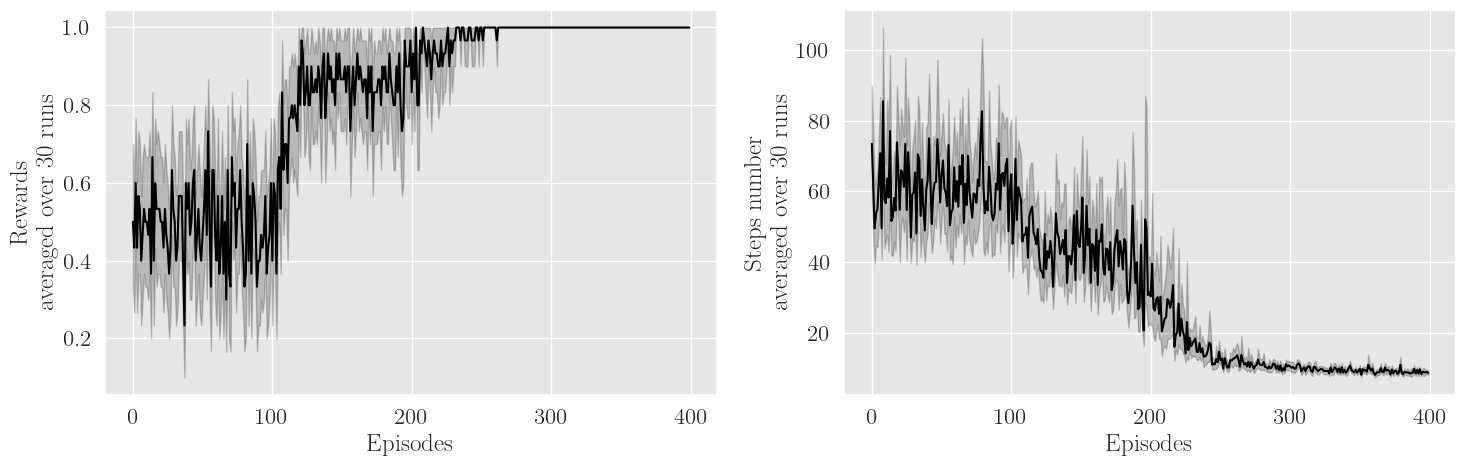
\includegraphics[height=0.35\textheight]{medias/steps-and-rewards-EastWest.png}
\end{center}
Left/Right
\begin{center}
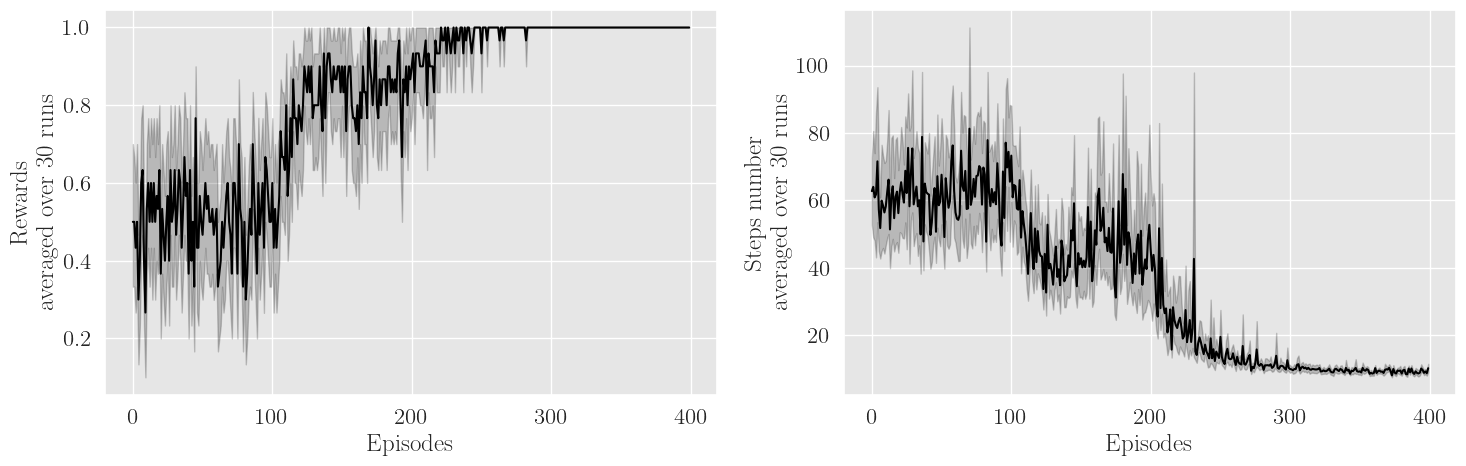
\includegraphics[height=0.35\textheight]{medias/steps-and-rewards-LeftRight.png}
\end{center}
\end{frame}
\begin{frame}[label={sec:orge47cf17}]{Training checks -- East/West}
\begin{center}
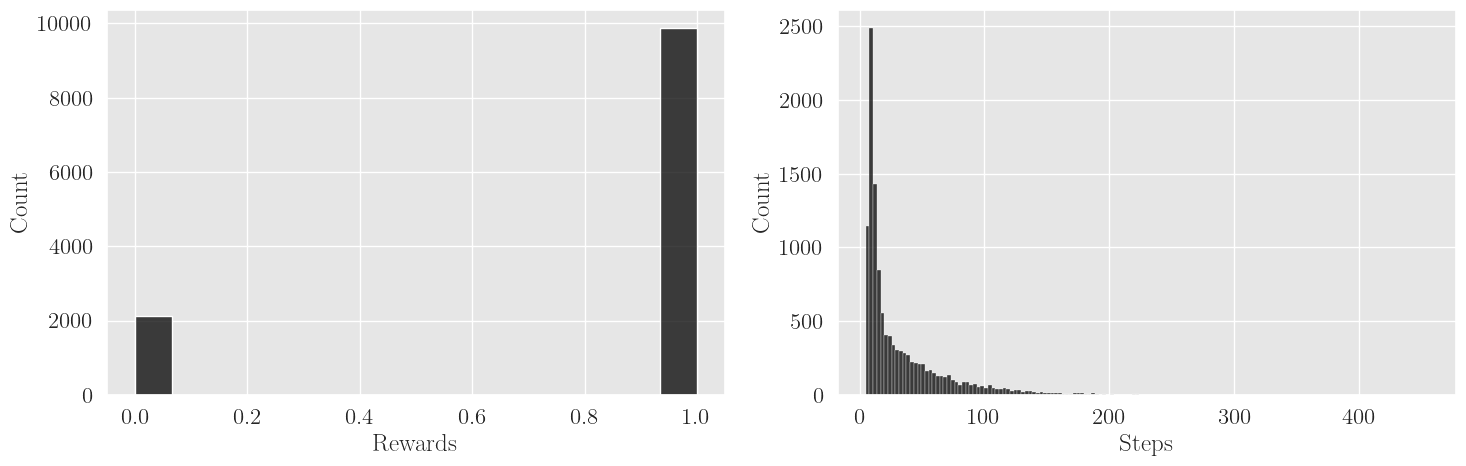
\includegraphics[width=\textwidth]{medias/steps-and-rewards-distrib-EastWest.png}
\end{center}
\begin{columns}
\begin{column}[c]{0.5\columnwidth}
\begin{center}
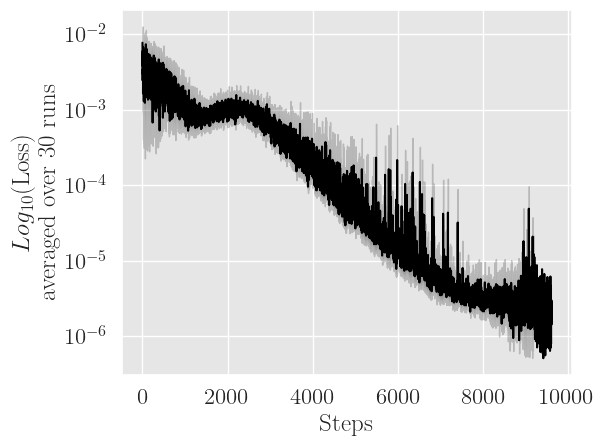
\includegraphics[width=0.8\textwidth]{medias/loss-EastWest.png}
\end{center}
\end{column}
\begin{column}[c]{0.5\columnwidth}
\begin{center}
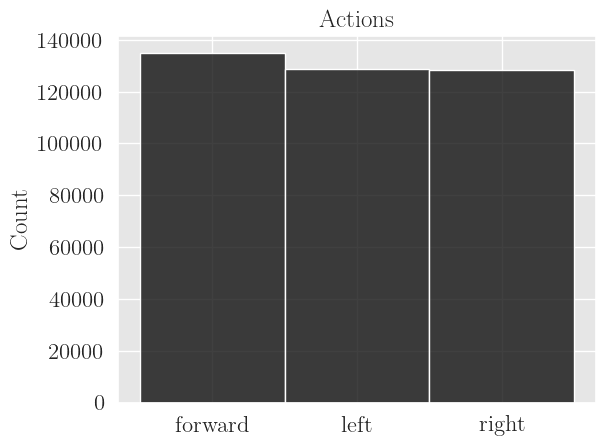
\includegraphics[width=0.65\textwidth]{medias/actions-distribution-EastWest.png}
\end{center}
\end{column}
\end{columns}
\end{frame}
\begin{frame}[label={sec:org098a8ed}]{Training checks -- Left/Right}
\begin{center}
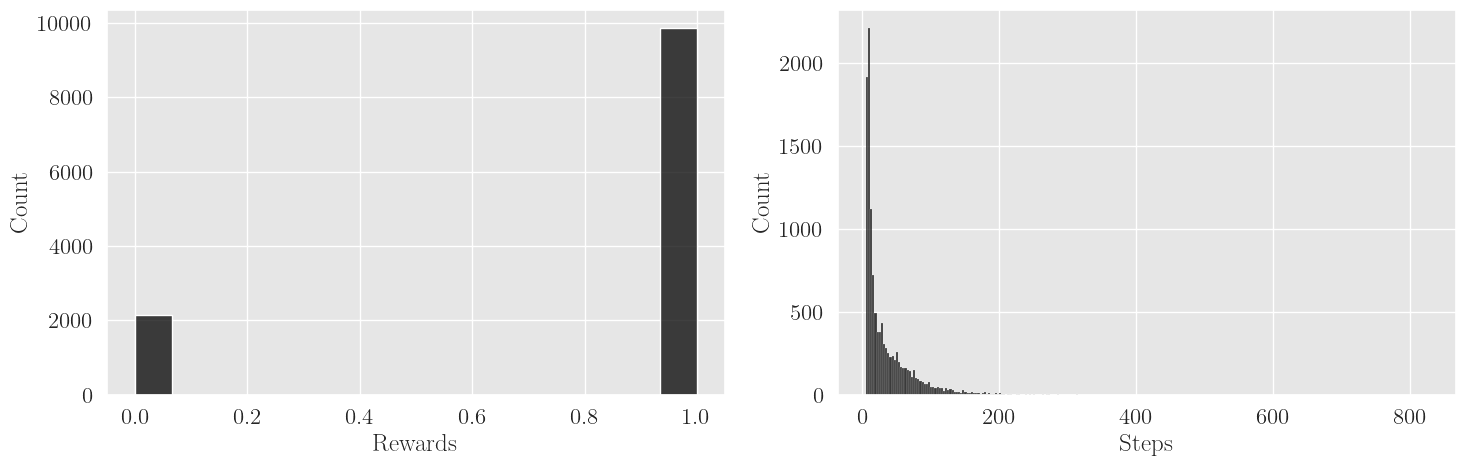
\includegraphics[width=\textwidth]{medias/steps-and-rewards-distrib-LeftRight.png}
\end{center}
\begin{columns}
\begin{column}[c]{0.5\columnwidth}
\begin{center}
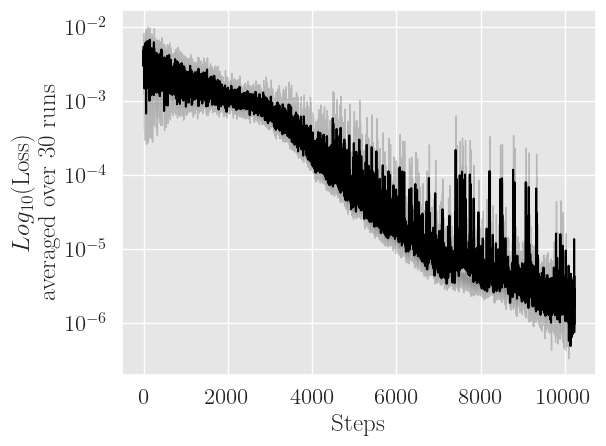
\includegraphics[width=0.8\textwidth]{medias/loss-LeftRight.png}
\end{center}
\end{column}
\begin{column}[c]{0.5\columnwidth}
\begin{center}
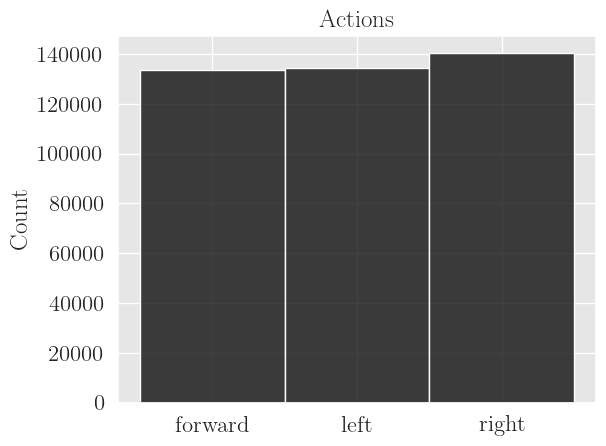
\includegraphics[width=0.65\textwidth]{medias/actions-distribution-LeftRight.png}
\end{center}
\end{column}
\end{columns}
\end{frame}
\begin{frame}[label={sec:org51ee38c}]{Agent behavior}
\begin{columns}
\begin{column}[c]{0.3\columnwidth}
\begin{center}
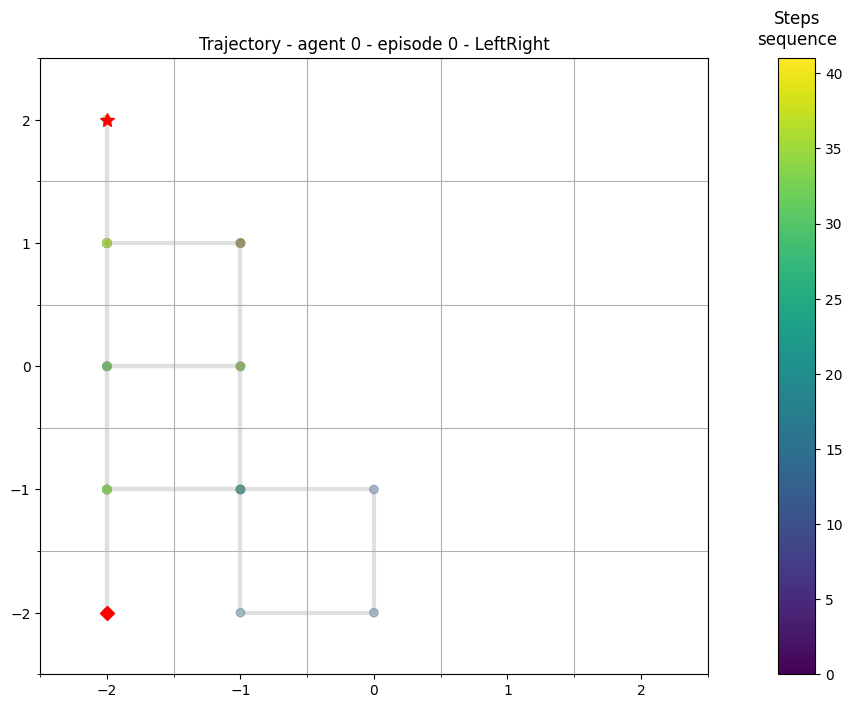
\includegraphics[height=0.28\textheight]{medias/trajectory-0-0-LeftRight.png}
\end{center}
\begin{center}
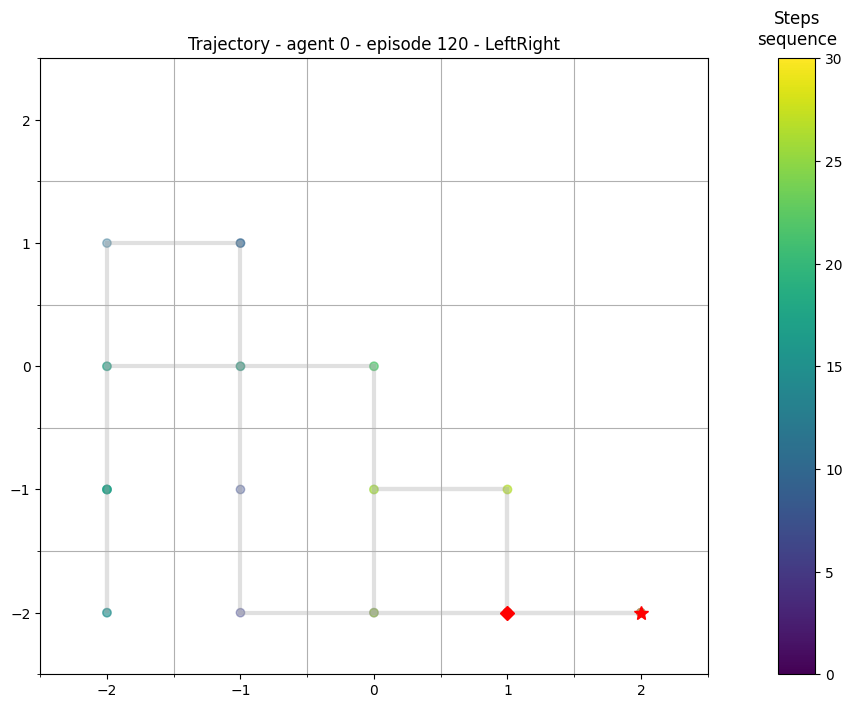
\includegraphics[height=0.28\textheight]{medias/trajectory-0-120-LeftRight.png}
\end{center}
\begin{center}
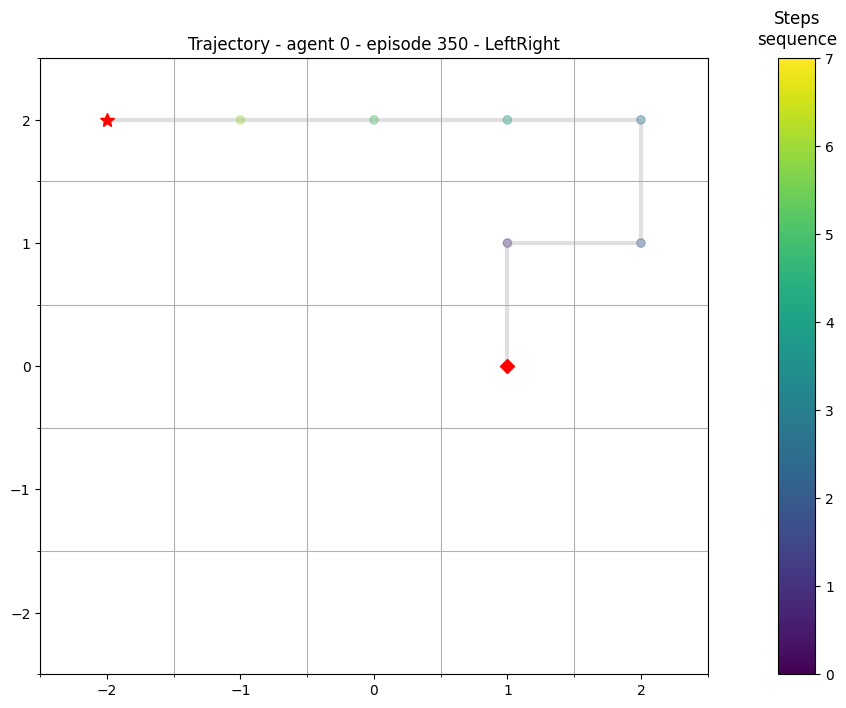
\includegraphics[height=0.28\textheight]{medias/trajectory-0-350-LeftRight.png}
\end{center}
\end{column}
\begin{column}[c]{0.3\columnwidth}
\begin{center}
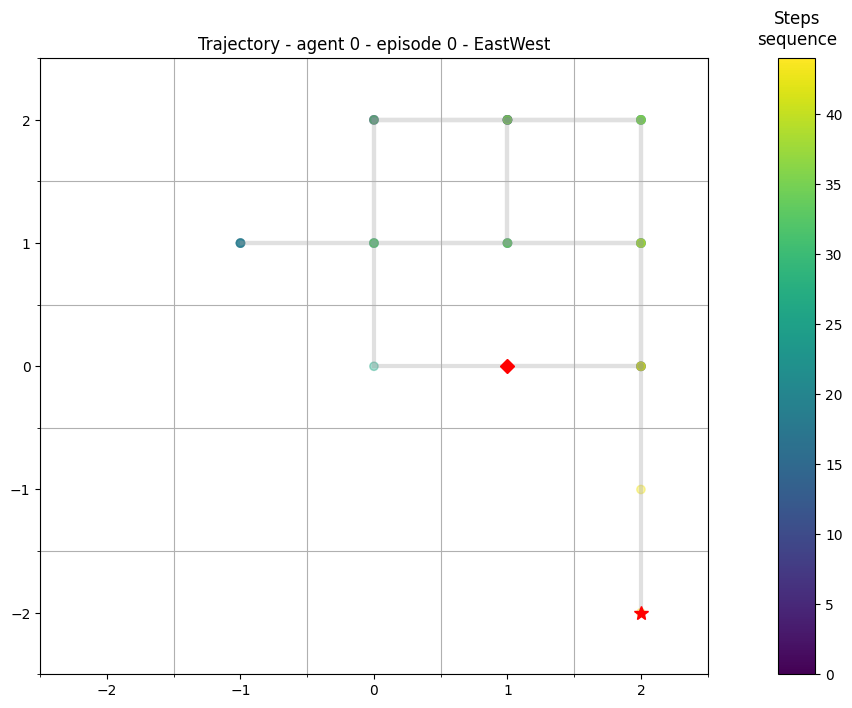
\includegraphics[height=0.28\textheight]{medias/trajectory-0-0-EastWest.png}
\end{center}
\begin{center}
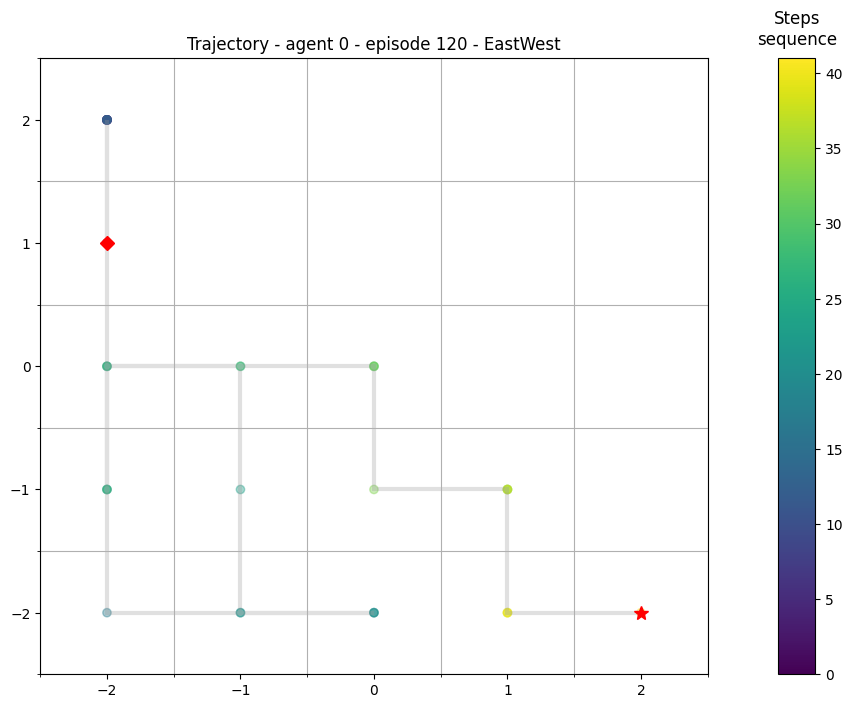
\includegraphics[height=0.28\textheight]{medias/trajectory-0-120-EastWest.png}
\end{center}
\begin{center}
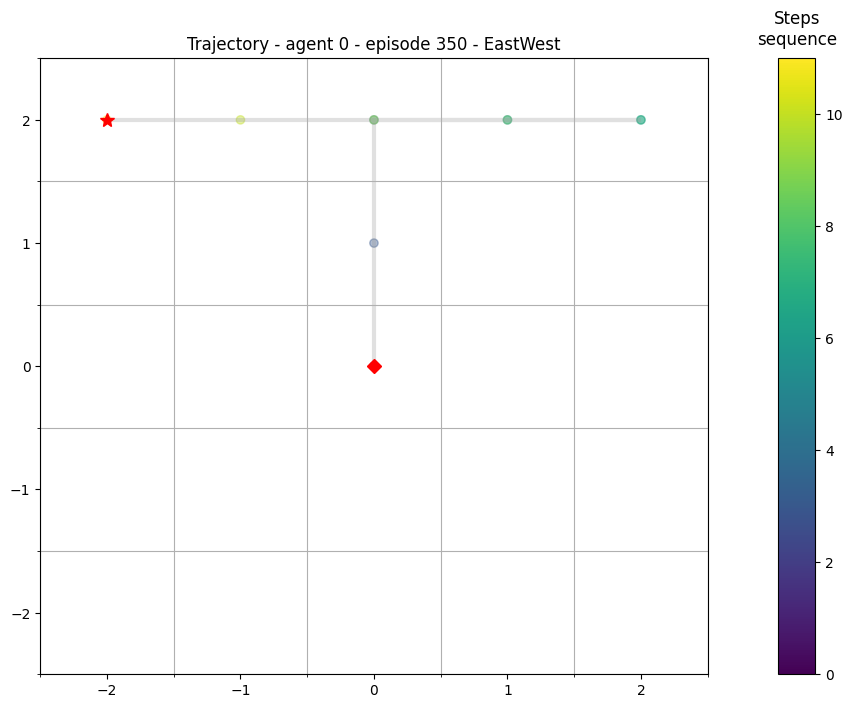
\includegraphics[height=0.28\textheight]{medias/trajectory-0-350-EastWest.png}
\end{center}
\end{column}
\end{columns}
\end{frame}
\section{What does the network learn?}
\label{sec:org9b6851d}
\begin{frame}[label={sec:org10049a3}]{Weights structure -- East/West}
\begin{center}
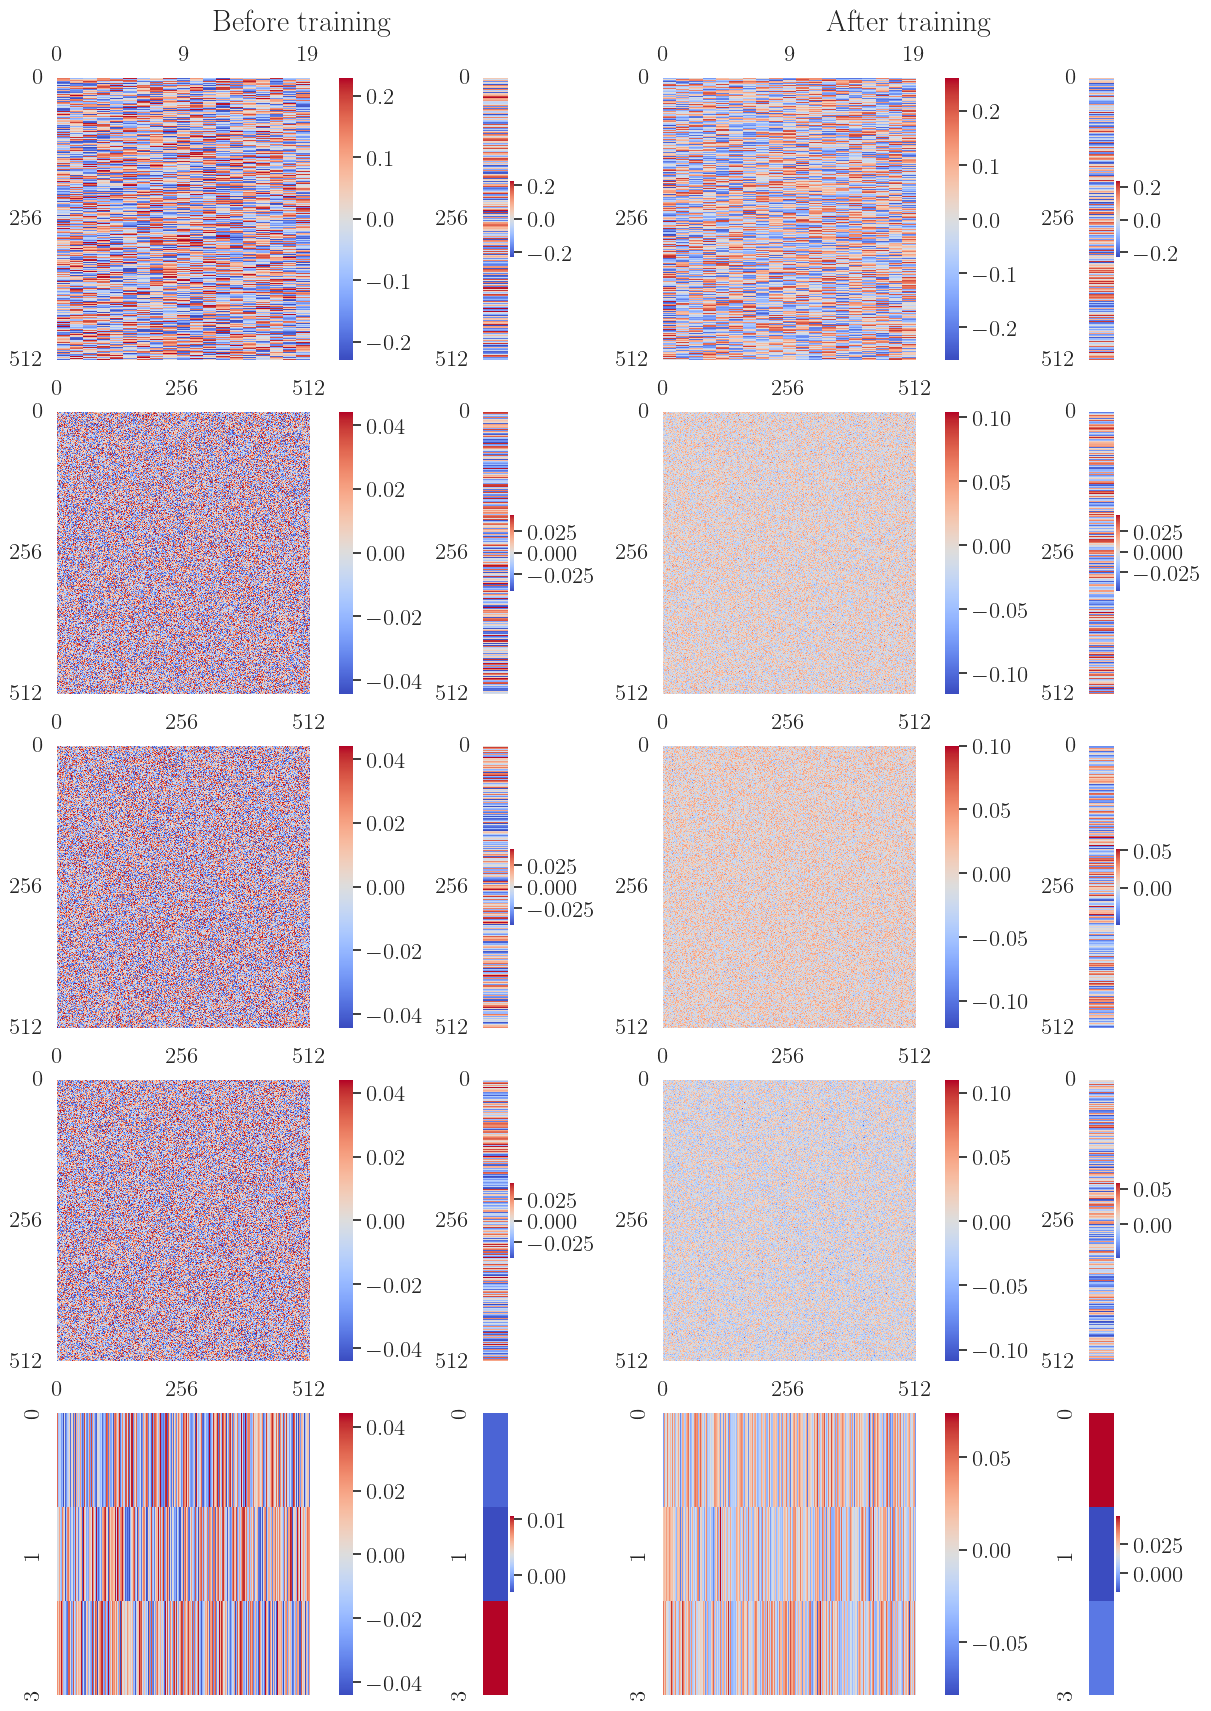
\includegraphics[height=0.96\textheight]{medias/weights-matrices-EastWest.png}
\end{center}
\end{frame}
\begin{frame}[label={sec:org00da435}]{Weights structure -- Left/Right}
\begin{center}
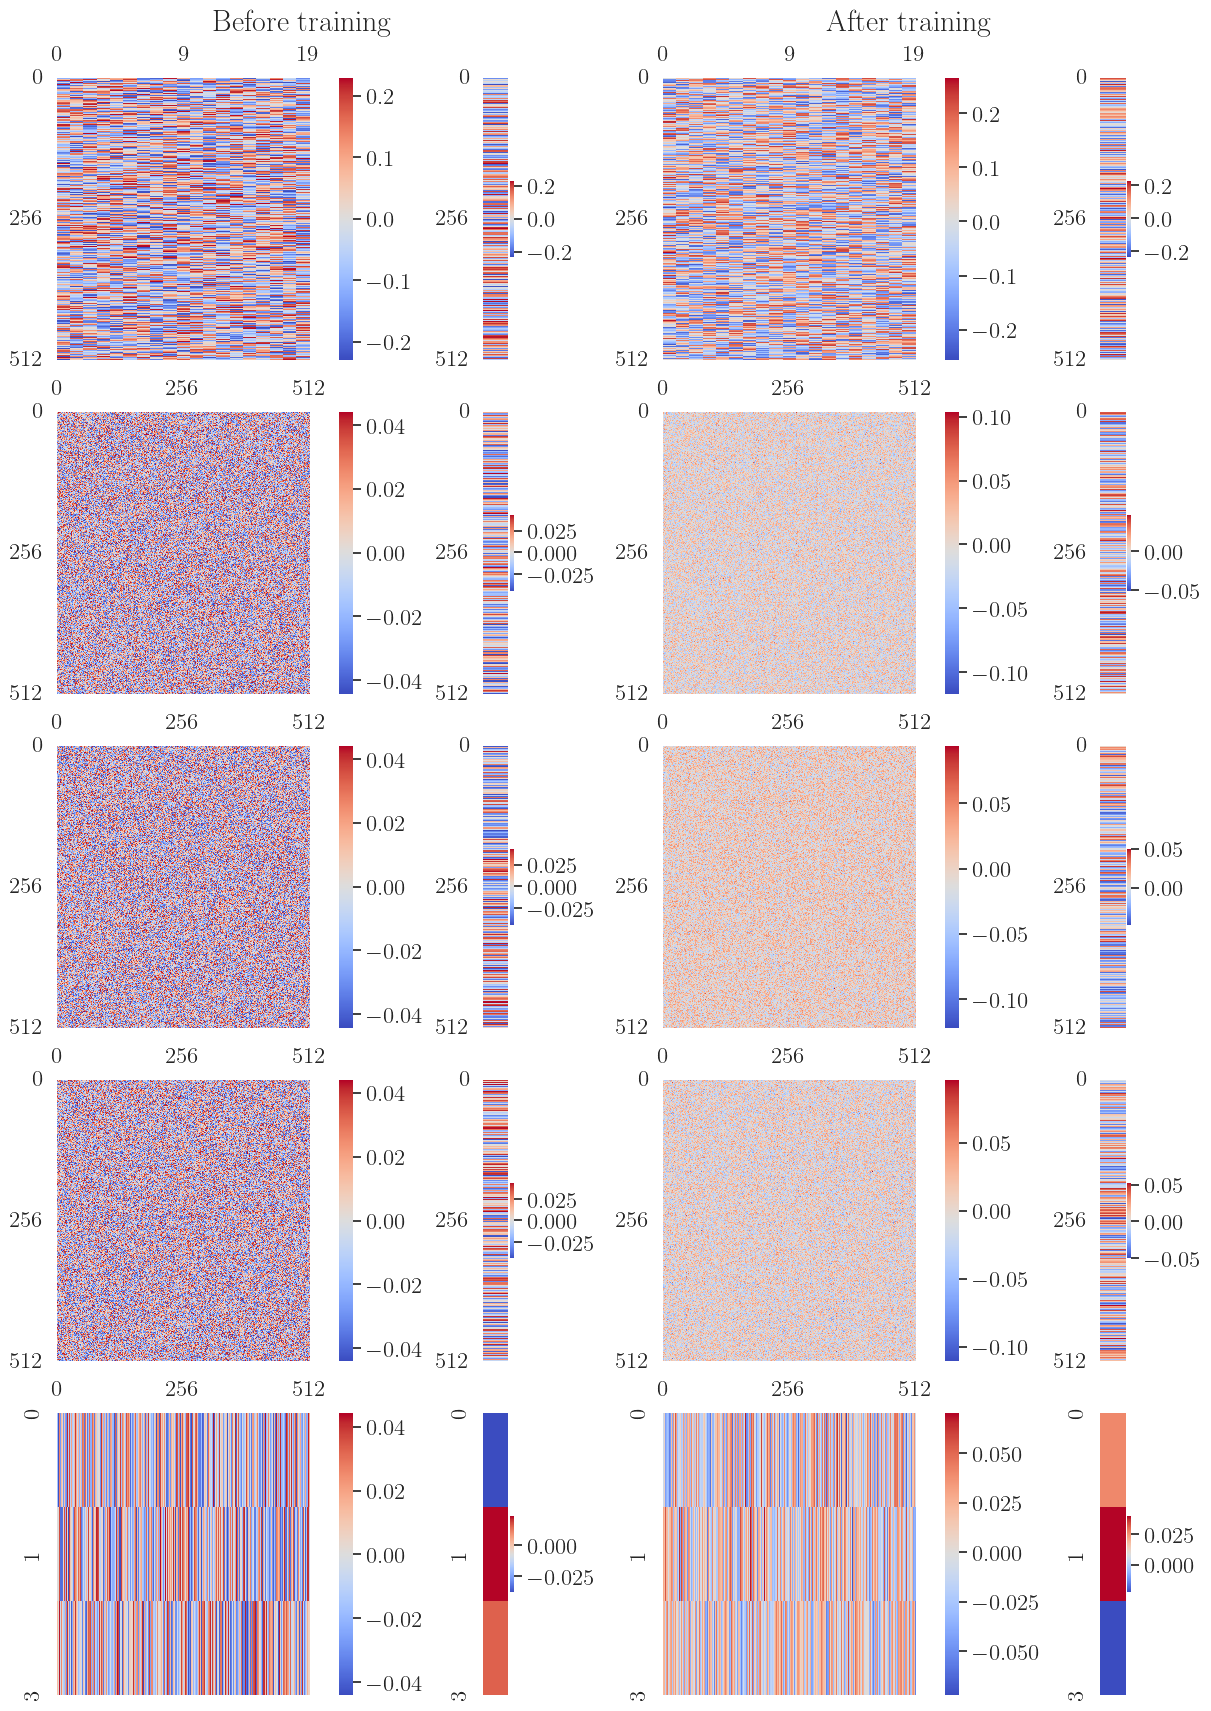
\includegraphics[height=0.96\textheight]{medias/weights-matrices-LeftRight.png}
\end{center}
\end{frame}
\begin{frame}[label={sec:org152ab71}]{Weights clustering}
\begin{center}
East/West
\end{center}
\begin{center}
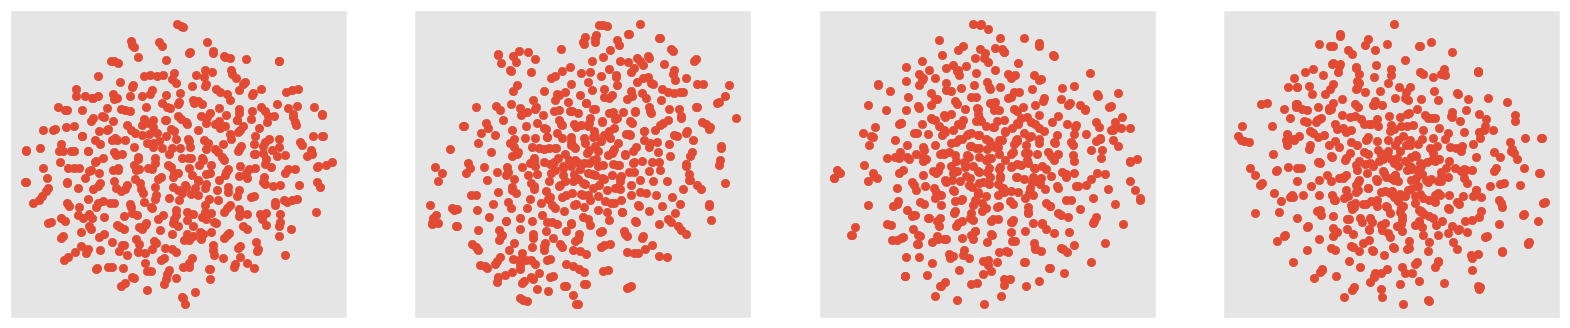
\includegraphics[width=.9\linewidth]{medias/weights-tSNE-EastWest.png}
\end{center}
\begin{center}
Left/Right
\end{center}
\begin{center}
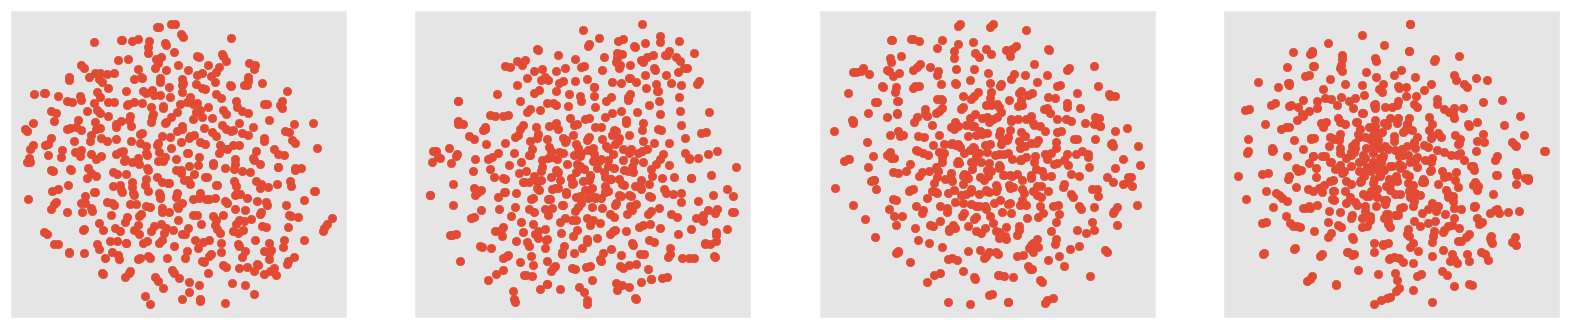
\includegraphics[width=.9\linewidth]{medias/weights-tSNE-LeftRight.png}
\end{center}
\end{frame}
\begin{frame}[label={sec:orga9c6d2b}]{Activations learned -- East/West}
\begin{center}
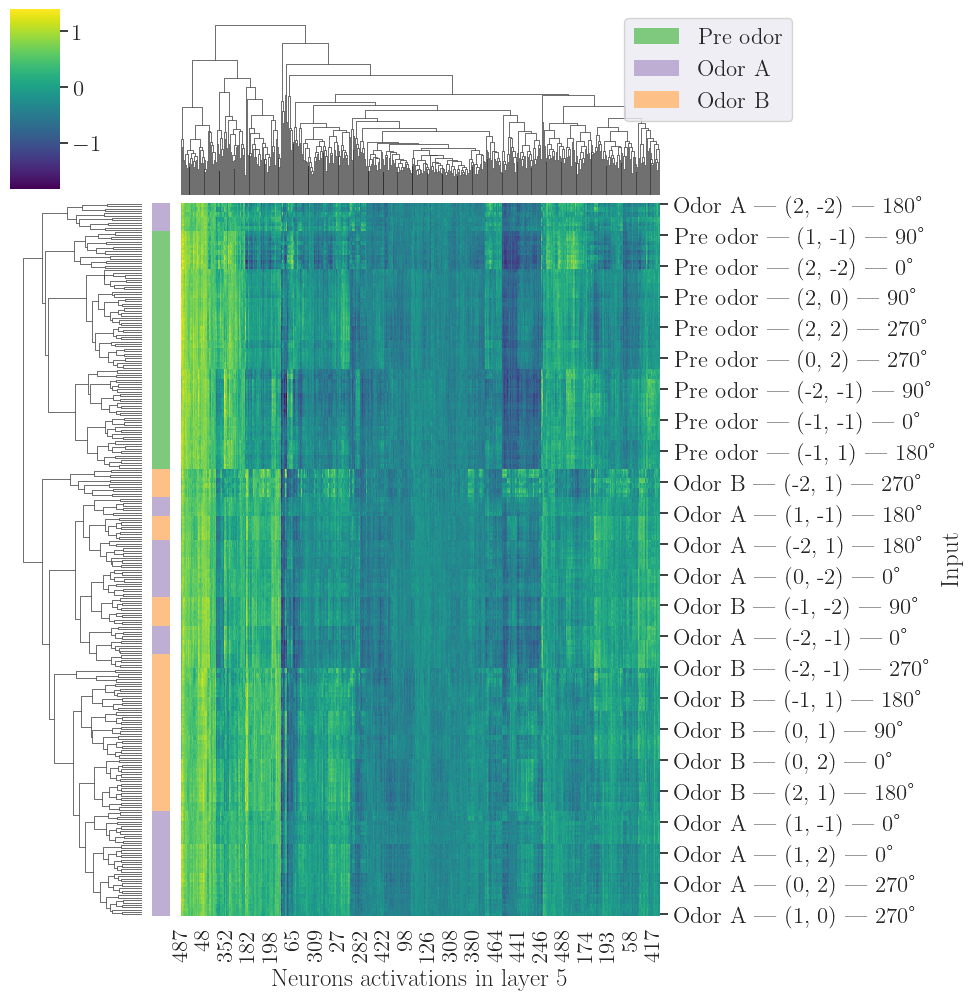
\includegraphics[height=0.9\textheight]{medias/activations-learned-EastWest.png}
\end{center}
\end{frame}
\begin{frame}[label={sec:org9b2cb18}]{Activations learned -- Left/Right}
\begin{center}
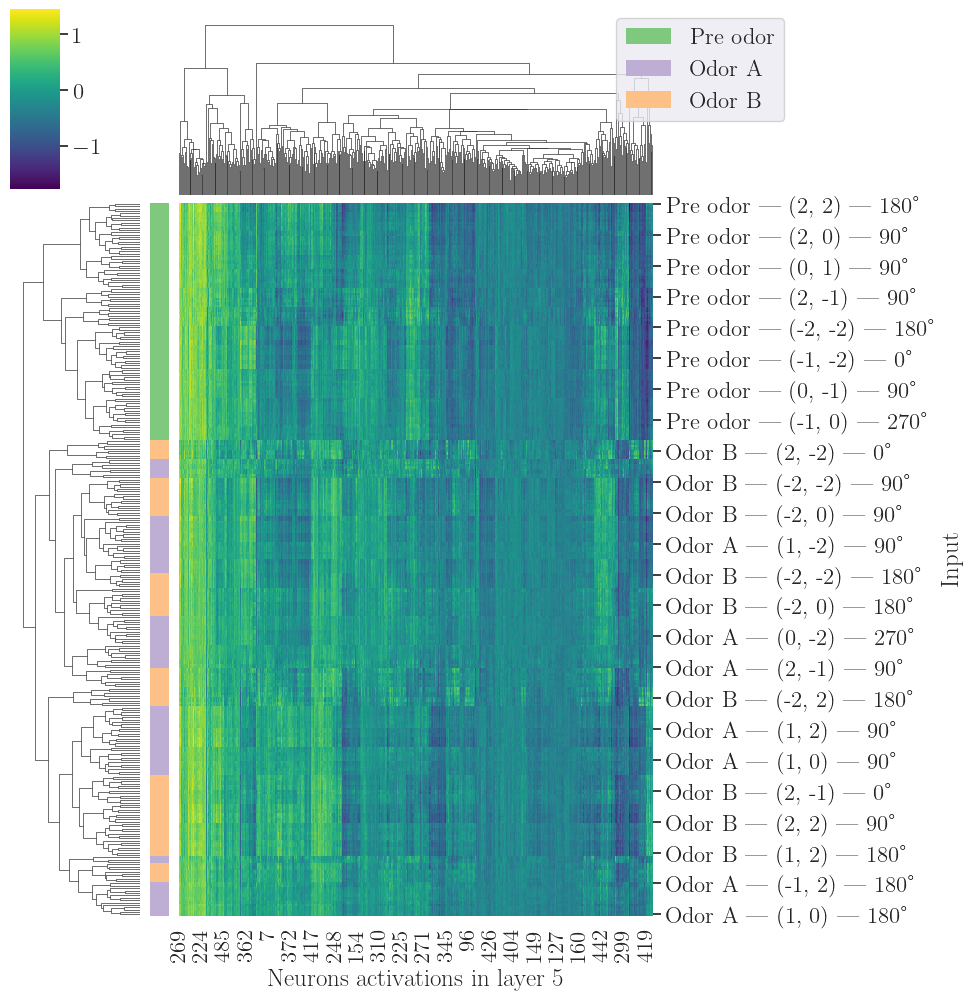
\includegraphics[height=0.9\textheight]{medias/activations-learned-LeftRight.png}
\end{center}
\end{frame}
\begin{frame}[<+->][label={sec:org34aa3ee}]{Use the behavior as proxy -- Perturbation experiment}
\begin{itemize}
\item Perturb the Cartesian/polar part of the input on a trained agent and look at how the agent behaves
\item Expectation:
\begin{itemize}
\item Left/right task:
\begin{itemize}
\item With the \alert{Cartesian} inputs perturbed \(\to\) agent's performance unchanged
\item With the \alert{polar} inputs perturbed \(\to\) agent's performance degrades
\end{itemize}
\item East/west task:
\begin{itemize}
\item With the \alert{polar} inputs perturbed \(\to\) agent's performance unchanged
\item With the \alert{Cartesian} inputs perturbed \(\to\) agent's performance degrades
\end{itemize}
\end{itemize}
\end{itemize}
\end{frame}
\begin{frame}[label={sec:orgf9da927}]{Cartesian inputs unchanged -- polar inputs perturbed}
\begin{columns}
\begin{column}[c]{0.5\columnwidth}
\begin{center}
\small
\textbf{East/West}\\
\footnotesize
Silencing inputs
\end{center}
\begin{center}
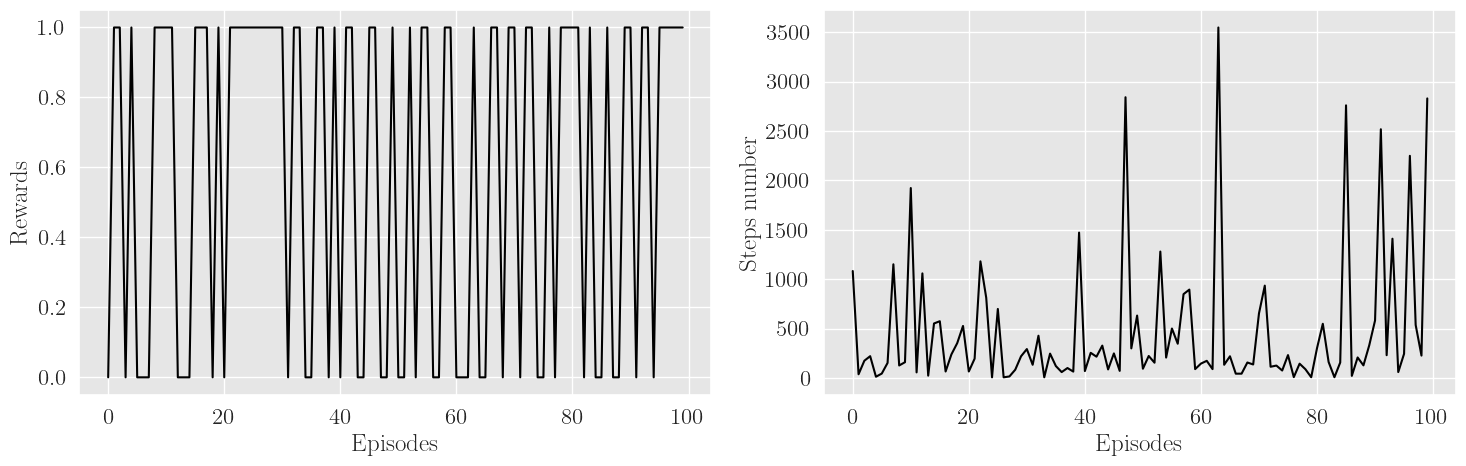
\includegraphics[width=\textwidth]{medias/steps-and-rewards-EastWest-perturb-silence.png}
\end{center}
\begin{center}
\footnotesize
Randomizing inputs
\end{center}
\begin{center}
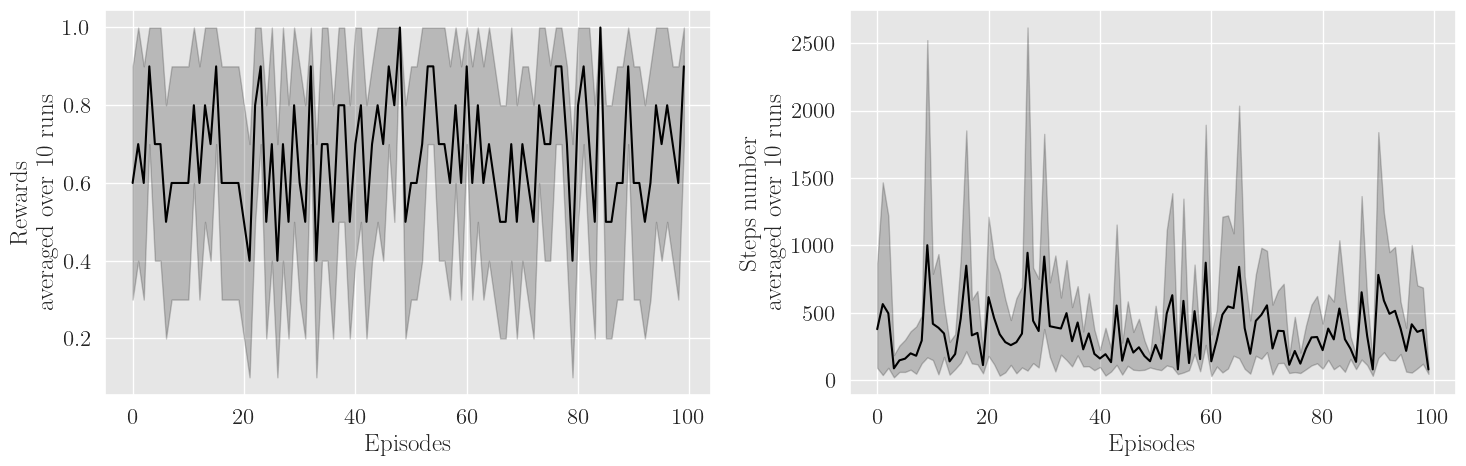
\includegraphics[width=\textwidth]{medias/steps-and-rewards-EastWest-perturb-rand.png}
\end{center}
\end{column}
\begin{column}[c]{0.5\columnwidth}
\begin{center}
\small
\textbf{Left/Right}\\
\footnotesize
Silencing inputs
\end{center}
\begin{center}
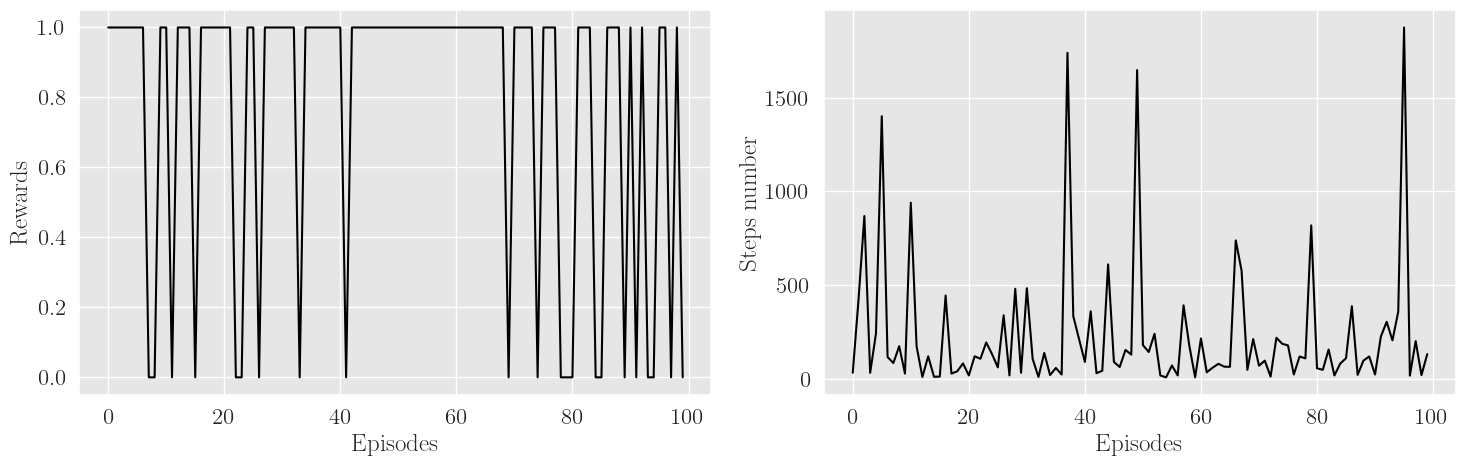
\includegraphics[width=\textwidth]{medias/steps-and-rewards-LeftRight-perturb-silence.png}
\end{center}
\begin{center}
\footnotesize
Randomizing inputs
\end{center}
\begin{center}
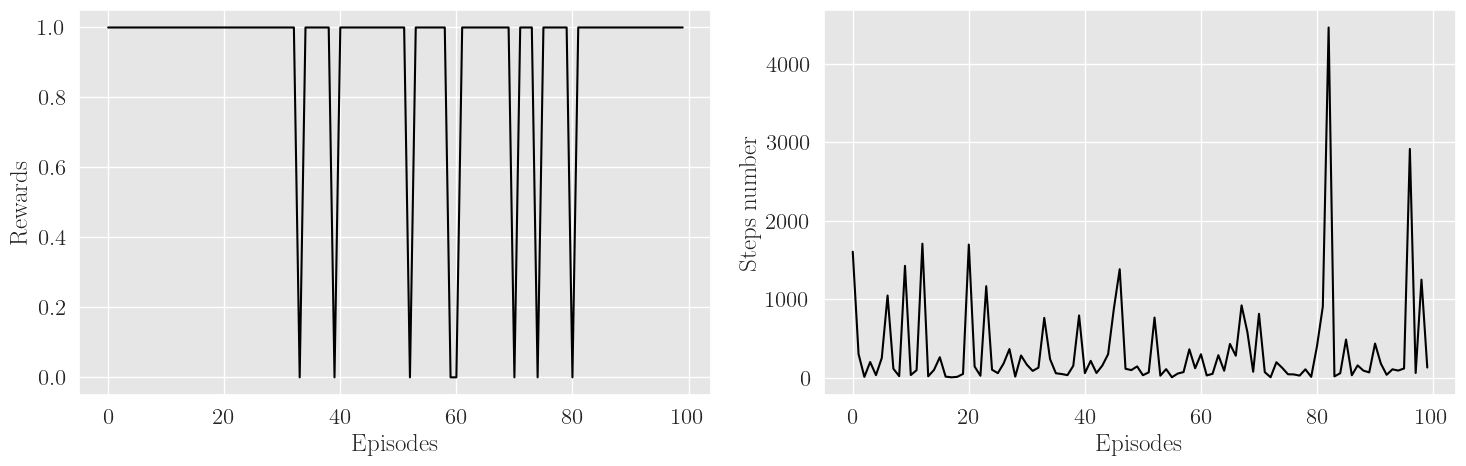
\includegraphics[width=\textwidth]{medias/steps-and-rewards-LeftRight-perturb-rand.png}
\end{center}
\end{column}
\end{columns}
\end{frame}
\begin{frame}[label={sec:orgad6cb04}]{Polar inputs unchanged -- Cartesian inputs perturbed}
\begin{itemize}
\item Simulation does not end

\(\to\) couldn't figure out why yet\(\dots\)
\end{itemize}
\end{frame}
\section{Conclusion}
\label{sec:orge121f0b}
\begin{frame}[<+->][label={sec:orga049cb2}]{Partial conclusions so far}
\begin{itemize}
\item \(\varnothing\) pattern on the weights
\item The \alert{pre-odor activations} cluster together, but no other clear pattern seems to emerge
\item So far with this task setup, it seems \alert{both types of coordinates information are required} to solve the task
\end{itemize}
\end{frame}
\begin{frame}[<+->][label={sec:orgb78fcef}]{Next steps}
\begin{itemize}
\item Perturbation experiment:
\begin{itemize}
\item Fix issue on Cartesian inputs
\item Setup more metrics for the study: performance histogram, \% correct, etc.
\end{itemize}
\item Need for some causal inference framework?
\item Use of techniques from explainable AI?
\item Study of the derivative of the output w.r.t. the inputs?
\item \alert{Timeline:} wrap the project by end of August
\end{itemize}
\end{frame}
\begin{frame}[label={sec:orgc74f247},standout]{~}
Questions ?
\end{frame}
\end{document}
